\documentclass[11pt]{article}
\usepackage[final]{acl}
\usepackage{times}
\usepackage{latexsym}
\usepackage[utf8]{inputenc}
\usepackage{microtype}
\usepackage{graphicx}
\usepackage{longtable}
\usepackage{booktabs}
\usepackage{array}

\providecommand{\tightlist}{%
  \setlength{\itemsep}{0pt}\setlength{\parskip}{0pt}}

\title{A/B Testing Performance Improvement Based on NLP Techniques: A Case Study of the Upworthy Research Archive}

\author{
  Damian Calabresi \and
  Jaeyeol You \and
  Hersh Rajesh Chawla \\
  University of Maryland, College Park
}

\begin{document}

\maketitle

\begin{abstract}
This project analyzes NLP techniques for predicting headline performance using the Upworthy Research Archive dataset. We compare traditional NLP methods (ranging from bi-grams to embeddings) with LLM-based approaches for click-through rate (CTR) prediction. Our analysis includes feature engineering, topic modeling using BERTopic, and evaluation of various linguistic features on headline success. We examine the relationship between sentiment, topic, readability, and other text characteristics with CTR, while controlling for confounders through A/B test analysis.
\end{abstract}

\section{Introduction}

A/B testing has become the gold standard for evaluating headline performance, allowing publishers to empirically compare different phrasings for the same article. The Upworthy Research Archive contains thousands of A/B tests of headlines done by Upworthy from January 2013 to April 2015 \cite{matias2021upworthy}. It provides a rich set of controlled experiments where different headlines were tested for the same articles. Each test provides click-through rate (CTR) data measured under randomized conditions allowing rigorous analysis of linguistic features affecting headline performance.

This project pursues two primary goals. First, we systematically validate hypotheses from recent literature suggesting that negative sentiment, headline length, and readability significantly impact CTR \cite{robertson2023negativity, munger2023linguistic}. Second, we compare the predictive performance of traditional NLP techniques with modern embedding approaches to determine whether semantic understanding captured by neural models provides advantages over surface-level linguistic features.

Our findings reveal important insights about the limitations of traditional NLP methods and the value of semantic representations. Notably, we challenge published findings regarding sentiment effects, finding no statistically significant correlation when using VADER sentiment analysis appropriate for short texts, despite multiple papers reporting significant negative sentiment effects using LIWC.

\section{Related Work}

Several studies have analyzed the Upworthy dataset to understand factors affecting headline success. The creator of the Upworthy Research Archive has done a meta analysis as part of his Princeton University course \cite{matias2020meta}, introducing key methodological contributions including de-meaning the data. The dataset contains the number of impressions and clicks for each headline. Comparing the click-rate between headlines in the dataset would be affected by the bias between articles. Some articles are more clickable than others (or were published at different hours). To control for this bias and do an intra-test comparison of the headlines, the mean of each test is subtracted from the headline CTR.

\textbf{Sentiment and Negativity.} Robertson et al. \cite{robertson2023negativity} found that negative words in news headlines increased consumption rates. For a headline of average length, each additional negative word increased the click-through rate by 2.3\%. Their techniques applied text mining, sentiment analysis done on the basis of the Linguistic Inquiry and Word Count (LIWC), Gunning Fog index for text complexity score, and multilevel binomial regression. Instead of applying a de-meaning to the headline CTR and then doing a linear regression, they applied a multi-level binomial regression to the data, fitting $logit(p_{ij}) = \alpha_j + \beta X_i$ where $p_{ij}$ is the probability of the headline $i$ in test $j$ to be clicked, with a different intercept coefficient alpha for each test.

Similarly, Gligorić et al. \cite{munger2023linguistic} examined linguistic effects on news headline success through thousands of online field experiments. They tested eight hypotheses in total and concluded that the presence of negative-emotion words is positively associated with headline success. Length and the use of first-person singular words are also positively associated with headline success. Their techniques applied logistic regression, word dictionaries for different categories, LIWC for the positive and negative emotion categories, and Flesch reading-ease score.

\textbf{Readability and Complexity.} Shulman et al. \cite{shulman2024reading} tested the hypothesis that writing that requires less effort to read will tend to be approached, liked, and engaged with. Their techniques applied a 24-item SDT paradigm to measure the reading difficulty of the headlines and LIWC score for the readability of the headlines. Thousands of field experiments across traditional (i.e., The Washington Post) and nontraditional news sites (i.e., Upworthy) showed that news readers are more likely to click on and engage with simple headlines than complex ones.

\textbf{Embedding and LLM Approaches.} Recent work has explored whether modern NLP techniques can predict or replace A/B testing. One study \cite{countbayesie2023gpt} examined whether GPT can predict the winner of an A/B test to avoid waiting for results and wasting conversions on poor-performing variants. They compared three embedding approaches: Bag-of-Words (bi-grams) with CountVectorizer, DistilBERT embeddings using Hugging Face Transformers library, and GPT-3 embeddings using OpenAI embeddings API. Logistic regression on the difference vector of embeddings (embedding\_a - embedding\_b) achieved 87\% accuracy with the GPT-3 model on the test set, while DistilBERT embeddings achieved approximately 80\% accuracy.

LOLA (LLM-Assisted Online Learning Algorithm) \cite{bastani2024lola} integrates LLM predictions into a bandit algorithm. They found standalone LLM predictions were only slightly above chance, but LOLA outperformed traditional A/B tests and pure bandits in simulations. Their techniques applied LLM as a classifier with few and zero-shot prompting, LLM-based CTR prediction model using LoRA fine-tuning, and LLM-Assisted 2-Upper Confidence Bounds (LLM-2UCBs). LOLA outperformed traditional A/B tests by 4-5\% and pure bandits by 2-3\% in simulations.

\textbf{Topic Modeling.} Jonsson et al. \cite{jonsson2021headline} examined headline sentiment and topic effect on online user engagement. They asked: What is the relationship between sentiment and click rate? Which topics lead to a higher click rate? How do variations in headline phrasing (tone, subjectivity) affect user behavior? Their techniques applied TextBlob for sentiment analysis to compute polarity and subjectivity of headlines, Latent Dirichlet Allocation (LDA) for topic modeling using Gensim library, and GSDMM (Gibbs Sampling algorithm for the Dirichlet Multinomial Mixture Model). They found that the sentiment of headlines (polarity and subjectivity) has little to no effect on click rate. The GSDMM model achieved acceptable coherence scores (0.46183) when using the top 5 words per topic.

\section{Methodology}

\subsection{Dataset}

The Upworthy Research Archive is a dataset of headlines tested by Upworthy.com with simple A/B testing to measure the performance and "catchy" factor of different headlines for the same news articles. It provides a list of news articles published, with different headlines tested for the same article. Each headline provides the number of impressions and clicks reached.

Upworthy is a website that publishes news articles and videos. It became one of the biggest news websites in the United States around 2013/2014, known for the ability to create viral content. Its popularity has been associated with the surge of Facebook and Twitter as social media platforms.

The dataset contains other columns like excerpt and share link, which are not visible in the Upworthy website and are only for social media sharing, which is not covered by the A/B testing.

\textbf{Terminology.} A \textit{package} is a headline being tested, a record in the dataset. It's considered a package because sometimes the eyecatcher picture varies but the headline is the same. A \textit{test} is a group of packages being tested, corresponding to one article for which different headlines were tested in a randomized setup.

\textbf{Data Preprocessing.} We stored a cleaned version of the dataset. In this dataset we only kept the tests where different headlines were used in the A/B tests. In addition, a flag has been added to identify the package with the highest CTR in the test.

Most of the articles tested contain between 4 and 6 packages. There are tests with up to 14 packages, but these may be exceptions. Some of these packages may contain the same headline test but different eyecatcher. Those packages were removed from further analysis.

\textbf{CTR De-meaning.} CTRs of different packages/headlines are not independent; each package is affected by confounders like the time of the day, the position in the website, and the content of the article. Within a test, the CTR of the packages are independent indeed, as this is the purpose of a randomized A/B test. To make every package CTR comparable, we de-meaned the CTR by the mean and standard deviation of the test. This means that the CTR of each package is now compared to the average CTR of the test. Figure~\ref{fig:ctr-demeaned} shows the distribution of de-meaned CTR values, centered around zero as expected.

\begin{figure}[h]
\centering
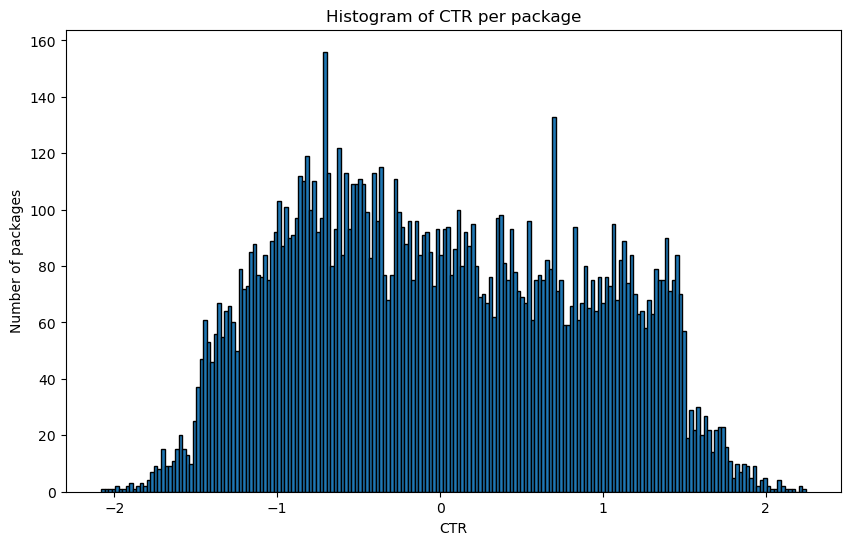
\includegraphics[width=0.9\columnwidth]{../images/ctr-demeaned-histogram.png}
\caption{Distribution of de-meaned CTR values. The histogram is centered around 0, with similar numbers of packages above and below 0, as expected from the normalization process.}
\label{fig:ctr-demeaned}
\end{figure}


\subsection{Feature Engineering}

After the exploration of the dataset has been done, the next step is to obtain new information from the dataset. The headline text is the main source of information, but the text alone would be difficult to analyze for a traditional predictor. Different features could be derived from the text, for example: Is a famous person mentioned in the headline? Does the headline use a specific English tense? Does the headline include a question? Nouns, verbs, words, and characters count. Sentiment analysis. Readability complexity score.

\textbf{Named-Entity Recognition.} Named-entity recognition (NER) is the process of identifying and extracting named entities from text. We used SpaCy to extract the named entities from the headlines. From the detected entities we considered the ones tagged as Person, Organization, and Geo-political Entity. Listing the names of people tagged shows that most of them are already famous people so we didn't require any further filtering. The following features were generated: \textit{headline\_num\_persons}, \textit{headline\_num\_orgs}, \textit{headline\_num\_gpes}, \textit{headline\_has\_person}, \textit{headline\_has\_org}, \textit{headline\_has\_gpe}.

\textbf{POS-based and Basic Text Features.} We also used SpaCy to extract the POS tags and identify different sentence characteristics that could potentially be useful for the analysis: \textit{starts\_with\_verb}, \textit{starts\_with\_pronoun}, \textit{starts\_with\_number} (whether the first content token is a verb, pronoun, or number); \textit{num\_chars}, \textit{num\_tokens}, \textit{avg\_token\_len} (basic length and tokenization statistics for the headline); \textit{ends\_with\_qmark}, \textit{ends\_with\_exclaim} (whether the headline ends with a question mark or exclamation mark); \textit{has\_quote}, \textit{has\_all\_caps\_word} (whether the headline contains any quote characters or a word in all caps); \textit{num\_nouns}, \textit{num\_verbs}, \textit{num\_adjs}, \textit{num\_advs}, \textit{num\_pronouns} (counts of nouns, verbs, adjectives, adverbs, and pronouns).

\textbf{Sentence Style Features.} One of the papers reviewed in the literature analyzed the sentence style of the headlines. We applied a custom approach to identify if the headline has an imperative style. It assumes that it's imperative if the root verb is in simple tense and there is no explicit subject related to it. The following feature was generated: \textit{headline\_imperative\_verb}.

\textbf{Curiosity and Intensity Features.} We came up with an approach to identify if the sentence expresses some intensity or curiosity. We identified a list of words commonly used in "curious" sentences or words that demonstrate intensity. Then we used the SpaCy embeddings similarity feature to identify if any of the words in the headline are similar to any of the words in the list. If they are, that similarity is indicated as the level of curiosity or intensity. The following features were generated: \textit{headline\_has\_curiosity\_word}, \textit{headline\_curiosity\_similarity}, \textit{headline\_has\_intensity\_word}, \textit{headline\_intensity\_similarity}.

\textbf{Sentiment Analysis.} The material "Negativity drives online news consumption (2023)" uses LIWC to analyze the sentiment of the headlines. LIWC is the most common method to analyze the sentiment of the text. We did research to understand how these methods work and found that LIWC is based on a sentiment dictionary and word counts. This makes it not very accurate for short texts like headlines. We used the VADER sentiment analysis tool from the NLTK library to analyze the sentiment of the headlines. VADER is a lexicon-based sentiment analysis tool that is designed to work with social media and short text in general. It makes focus on punctuation, capitalization, and word context in short sentences. Using this method, the following features were generated: \textit{neg} (negative sentiment score), \textit{neu} (neutral sentiment score), \textit{pos} (positive sentiment score), and \textit{compound} (compound sentiment score that varies from -1 to 1, where -1 is very negative, 0 is neutral, and 1 is very positive).

\textbf{Dataset Related Features.} We also generated some features that could be helpful in the prediction of the CTR: \textit{created\_at\_dayofweek}, \textit{created\_at\_hourofday}, \textit{test\_group\_size}.

\textbf{Readability Features.} We used the Flesch Reading Ease and Coleman–Liau index scores as two alternative readability measures. We applied both of them as Flesch Reading Ease score is based on the number of syllables in the words and it may not be very accurate for short texts like headlines. Coleman–Liau index is based on the number of characters per word and may be better for short texts. The paper "Linguistic effects on news headline success: Evidence from thousands of online field experiments (2023)" uses the Flesch Reading Ease score to measure the readability of the headlines. The following features were generated: \textit{read\_flesch}, \textit{read\_coleman}.

\textbf{Specificity Feature.} To calculate the specificity of the headline, first we generated a corpus based on the entire dataset. Then we used the Scikit-learn TF-IDF vectorizer to calculate the TF-IDF score for each headline and each word. The inclusion of infrequent words is supposed to increase the specificity of a headline compared to others. The result was stored in the feature \textit{specificity\_tfidf}.

\subsection{Topic Modeling}

To understand how different features affect the CTR we may also need to control for the topic of the headline, as different topics may have a different audience. We analyzed different algorithms for topic modeling.

\textbf{Latent Dirichlet Allocation (LDA).} LDA (Latent Dirichlet Allocation) is an unsupervised topic modeling technique that is used to identify the topics in a corpus of text. It is a Bayesian probabilistic model based on mixture of words. For this reason, it's fitted for large corpora of text and not well suited for short texts like headlines.

\textbf{GSDMM (Gibbs Sampling Dirichlet Multinomial Mixture).} GSDMM is a clustering algorithm designed for short texts like headlines. It assumes each text belongs to only one of K topics. The algorithm groups similar texts together by maximizing both topic similarity and topic size.

\textbf{BERTopic.} BERTopic is the state-of-the-art topic modeling technique. It uses BERT embeddings to represent the text. Its pipeline is defined by these steps: Embedding, Dimensionality reduction, Clustering, Tokenization, Weighting Scheme, and Representation Tuning (This stage is optional and we're not going to use it).

We chose to use BERTopic for topic modeling as it's the state-of-the-art technique and its practical for small datasets.

\section{Results}

\subsection{Feature Impact on CTR}

CTR prediction has been done using a linear regression. The analysis of the engineered features and their statistical significance gave us the following results:

\textbf{Named entities:} There is no correlation with the CTR.

\textbf{Sentence starting, Question/Exclamation features:} Headlines starting with a verb, with question or exclamation marks are associated with a lower CTR, this isn't something we expected.

\textbf{Basic text features:} Definitively there is a correlation with the number of pronouns.

\textbf{Sentence style:} A mild correlation with the use of specific intensity words.

\textbf{Sentiment:} Contrary to what we expected, based on the reviewed literature, there is no correlation with the sentiment of the headline at all.

\textbf{Specificity:} The use of specific words is associated with a decrease in the CTR.

These results were obtained doing a linear regression over the engineered features in the exploratory and confirmatory datasets. Regressions were run for all the features simultaneously and then for groups of features to avoid multicollinearity issues.

Table~\ref{tab:feature-impact} shows the p-value and confidence interval for each feature taken as relevant.

\begin{table*}[t!]
\centering
\small
\begin{tabular}{lrrrrrc}
\toprule
Feature & coef & std err & t & P$>|$t$|$ & [0.025 & 0.975] \\
\midrule
starts\_with\_verb & -0.0679 & 0.012 & -5.615 & 0.000 & -0.092 & -0.044 \\
starts\_with\_pronoun & 0.0254 & 0.009 & 2.869 & 0.004 & 0.008 & 0.043 \\
num\_pronouns & 0.0228 & 0.004 & 6.131 & 0.000 & 0.016 & 0.030 \\
ends\_with\_qmark & -0.1967 & 0.013 & -14.926 & 0.000 & -0.223 & -0.171 \\
ends\_with\_exclaim & -0.2211 & 0.037 & -5.953 & 0.000 & -0.294 & -0.148 \\
headline\_has\_intensity\_word & 0.0315 & 0.011 & 2.890 & 0.004 & 0.010 & 0.053 \\
headline\_intensity\_similarity & 4.5559 & 2.082 & 2.188 & 0.029 & 0.475 & 8.636 \\
neg & 26.4455 & 15.158 & 1.745 & 0.081 & -3.265 & 56.156 \\
neu & 26.3195 & 15.159 & 1.736 & 0.083 & -3.392 & 56.031 \\
pos & 26.1057 & 15.159 & 1.722 & 0.085 & -3.607 & 55.818 \\
compound & 0.0085 & 0.032 & 0.265 & 0.791 & -0.054 & 0.071 \\
specificity\_tfidf & -0.5161 & 0.061 & -8.496 & 0.000 & -0.635 & -0.397 \\
\bottomrule
\end{tabular}
\caption{P-value and confidence interval for features with significant or near-significant effects on CTR.}
\label{tab:feature-impact}
\end{table*}


\subsection{Topic Modeling Results}

BERTopic assigned 50\% of the headlines to a topic. Based on the top words of each topic, we titled the first 18 topics as follows: (--1) Miscellaneous, (0) She, He, Pronouns, (1) Kids, (2) Food \& Restaurants, (3) Racism, (4) Gay Marriage, (5) Feminism, (6) Science \& Medicine, (7) Pets \& Animals, (8) Music, (9) Crime, (10) Water \& City, (11) Guns \& Wars, (12) Money \& Economy, (13) Fashion, (14) Climate Change, (15) Space, (16) Viral Videos \& Content, (17) Men (He, Him, His), (18) Future \& Predictions.

\textbf{CTR Prediction per Topic.} We ran a linear regression for each topic separately. The results are not statistically significant for any of the topics due to the small number of headlines per topic.

\subsection{Literature Validation}

Two published and peer-reviewed papers confirmed that a negative sentiment is associated with a higher CTR. Those methods use LIWC for sentiment analysis which, as explained before (and it's confirmed in the LIWC website), are not good for short texts like headlines. When applying VADER sentiment analysis to the headlines, the correlation is not statistically significant.

This is of upmost importance given that the article "Negativity drives online news consumption (Robertson et al., 2023)" was published in Nature, has been peer reviewed, cited multiple times, and this outcome has been in news sites. We found peer reviewed validations of this research but they don't discuss the accuracy of LIWC to measure the negativity and positivity of the headlines.

Our results partially contradict published findings on sentiment. While \citet{robertson2023negativity} and \citet{munger2023linguistic} found significant negative sentiment effects using LIWC, our VADER-based analysis found no statistically significant correlation. This discrepancy seems to be related to the use of different sentiment analysis tools (LIWC vs. VADER).

\section{Headline Success Prediction}

\subsection{Traditional NLP Techniques}

We conducted a rigorous benchmark using state-of-the-art Traditional NLP methods, testing various strategies to handle the extreme class imbalance (95\% Losers vs. 5\% Winners).

\textbf{Key Findings.} When we applied a high class weight ($\sim$18.5), the model over-predicted winners (10,000+), sacrificing precision. When we reduced the weight, the model became too conservative, predicting almost zero winners (only 9). This "Swing" phenomenon proves that the model cannot distinguish true winners from losers; it merely biases its guessing strategy based on the weight.

\textbf{The "Random Guess" Baseline.} Across all experiments, the ROC-AUC score remained stagnant near 0.5 (0.54). This quantitatively confirms that headline success is not linearly correlated with surface-level linguistic features (TF-IDF, sentiment, readability).

\textbf{Strategic Implication.} This failure is our most important insight. It demonstrates that the "Curiosity Gap" is a semantic nuance invisible to traditional statistical models. Traditional NLP counts words (e.g., "Does 'video' appear?"), while Generative AI (LLM) understands intent (e.g., "Does this headline create a question in the reader's mind?"). Therefore, this benchmark provides the definitive data-driven justification for our team's transition to GPT-based approaches.

\subsection{Embedding Techniques}

We used embeddings to predict the success of a headline. The process compared two minimal embedding models: All-MiniLM-L6-v2 and BAAI/bge-base-en-v1.5. The results were: All-MiniLM-L6-v2 achieved 60\% accuracy and BAAI/bge-base-en-v1.5 achieved 63\% accuracy.

The embedding obtained for each headline were transformed into a difference vector and this vector was used to train a Linear Regression and a Neural Network. The difference between those two models was minimal.

From the experiments we can conclude that even simple embedding models provide a better result than traditional NLP techniques, and the embedding technique as well as the model is more important in the result than the machine learning model used.

\section{Conclusion}

Our most significant finding challenges widely-cited research on sentiment effects. While peer-reviewed papers published in Nature and PLOS ONE reported that negative sentiment significantly increases CTR using LIWC-based analysis, our VADER-based sentiment analysis-which is specifically designed for short texts-found no statistically significant correlation. This discrepancy highlights a critical methodological consideration: LIWC, as acknowledged on its official website, is not appropriate for texts with fewer than 10 words, yet headlines average usually below or near to this threshold. This finding calls for re-examination of sentiment effects in headline optimization using methods appropriate for short-form text.

Our feature engineering revealed several significant linguistic patterns. Headlines starting with verbs or ending with question marks are associated with lower CTR, contrary to conventional wisdom. The number of pronouns shows positive correlation with CTR, and the use of specific intensity words shows mild positive effects. However, specificity (measured by TF-IDF) is associated with decreased CTR. These findings provide actionable insights for content optimization.

The headline success prediction experiments demonstrate a fundamental limitation of traditional NLP approaches. Despite comprehensive feature engineering, traditional methods achieved near-random performance (ROC-AUC $\sim$0.54). This failure reveals that headline success depends on semantic nuances that surface-level features cannot capture.

In contrast, even simple embedding-based approaches (All-MiniLM-L6-v2 and BAAI/bge-base-en-v1.5) achieved 60-63\% accuracy, substantially outperforming traditional methods. This demonstrates that semantic representations captured by transformer models provide advantages over surface-level linguistic features. The choice of embedding model matters more than the subsequent machine learning architecture.

These results have important practical implications. Publishers seeking to optimize headlines should invest in semantic understanding technologies rather than relying solely on surface-level features. Future work should explore fine-tuned language models and investigate whether LLM-assisted approaches like LOLA can further improve upon pure embedding methods in real-world deployment scenarios.

\section*{Acknowledgments}

We thank the course instructor for his guidance throughout this project. We also acknowledge Nathan Matias for creating and maintaining the Upworthy Research Archive dataset.

\bibliographystyle{acl_natbib}
\bibliography{custom}

\end{document}
